
\documentclass[3p]{elsarticle}
\journal{}

\usepackage{graphicx}
\usepackage{amsmath}
\usepackage{amssymb}
\usepackage{amsthm}
\usepackage{latexsym}
\usepackage{bm}
\usepackage{array,supertabular}
\usepackage{color}
\usepackage{framed}
\usepackage{setspace}
\usepackage{fancyhdr}
\usepackage{stmaryrd}
\usepackage{mathrsfs}
\usepackage{mdframed}
\usepackage{url}
\usepackage{ctex}
\usepackage{algorithm}
\usepackage{algpseudocode}

\SetSymbolFont{stmry}{bold}{U}{stmry}{m}{n}

\newtheorem{defi}{Definition}
\newtheorem{lemma}{Lemma}
\newtheorem{proposition}{Proposition}
\newtheorem{remark}{Remark}

\numberwithin{equation}{section}

\newenvironment{myenv}[1]
{\mdfsetup{
		frametitle={\colorbox{white}{\space#1\space}},
		innertopmargin=10pt,
		frametitleaboveskip=-\ht\strutbox,
		frametitlealignment=\center
	}
	\begin{mdframed}
	}
	{\end{mdframed}}

\begin{document}
	
	\begin{frontmatter}
		
		\title{\textbf{MAE 5032 HPC Final Project --  the transient heat equation in a one-dimensional (1D) domain}}
		\author{Jiayi Huang}
		
		\begin{abstract}
			本文利用有限差分法计算热方程的数值解,在一个一维热方程的具体问题中,使用显示欧拉法和隐式欧拉法分别求解,两种求解均基于PETsC库。根据逐步加细的网格和逐步减小的时间步长,分析并计算了截断误差如何依赖于网格间距和时间步长,并给出理论预测。
		\end{abstract}
		
		\begin{keyword}
			 Finite difference method, Explicit Euler and Implicit Euler methods
		\end{keyword}
	\end{frontmatter}
	
	\section{Introduction}
    首先列出要求解的一维传热问题
    
    \begin{aligned}
    	\rho c \frac{\partial u}{\partial t}-\kappa \frac{\partial^{2} u}{\partial x^{2}} &=f & & \text { on } \Omega \times(0, T) \\
    	u &=g & & \text { on } \Gamma_{g} \times(0, T) \\
    	\kappa \frac{\partial u}{\partial x} n_{x} &=h & & \text { on } \Gamma_{h} \times(0, T) \\
    	\left.u\right|_{t=0} &=u_{0} & & \text { in } \Omega . 
    \end{aligned}

    其中 $u = u(x,t)$ 是要求解的 $t$ 时刻,$x$ 位置处的温度。可以画出下面的示意网格。
    
    \begin{figure}[h]
	\begin{center}
		\begin{tabular}{c}
			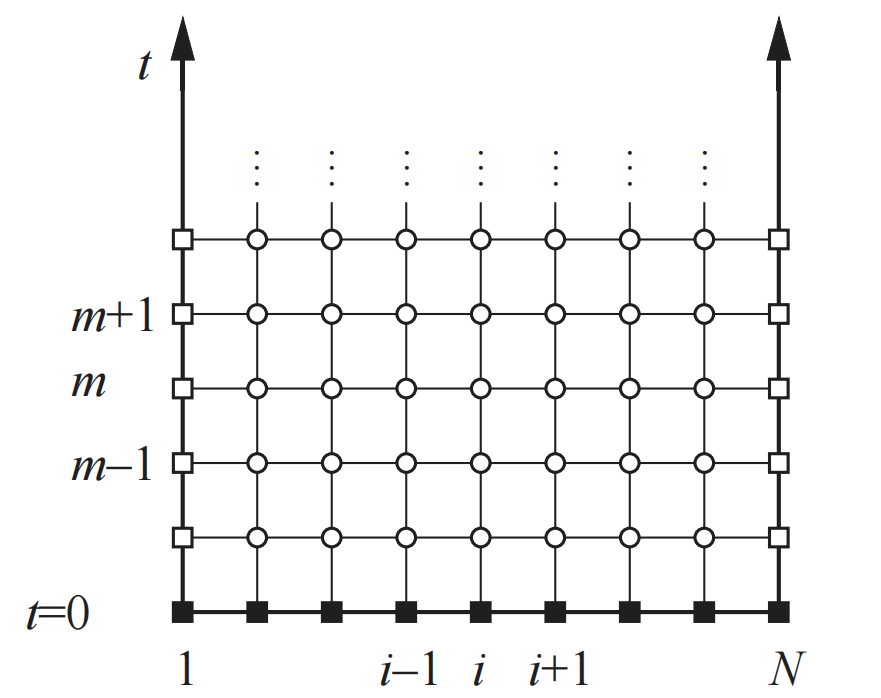
\includegraphics[angle=0, clip=true, scale=0.25]{./figures/mesh.png}
		\end{tabular}
	\end{center}
	\caption{解一维热方程的示意网格,实心方块代表已知位置,空心的则代表用有限差分近似的位置}
	\label{fig:illustration-mesh}
    \end{figure}
    
    
    \begin{figure}[h]
    	\begin{center}
    		\begin{tabular}{c}
    			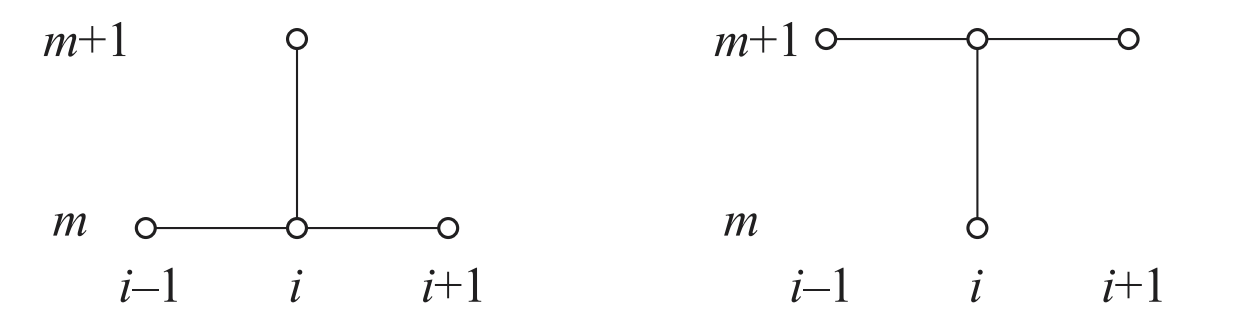
\includegraphics[angle=0, clip=true, scale=0.25]{./figures/compute_molecules.png}
    		\end{tabular}
    	\end{center}
    	\caption{关于有限差分的计算子,左边是Explicit Euler,右边是Implicit Euler}
    	\label{fig:illustration-molecules}
    \end{figure}

    根据上面的差分算子示意图,可以推导出下面的两个 Explicit Euler 和 Implicit Euler 迭代公式。
        
	\begin{equation}
		u_{i}^{m+1}=\alpha u_{i+1}^{m}+(1-2 \alpha) u_{i}^{m}+\alpha u_{i-1}^{m} + \beta \cdot f
	\end{equation}

	\begin{equation}
	    u_{i}^{m-1} = -\alpha u_{i+1}^{m}+(1+2 \alpha) u_{i}^{m}-\alpha u_{i-1}^{m} - \beta \cdot f
	\end{equation}

    其中 $ \alpha =  \kappa \beta / \Delta x^{2} $ , $ \beta = \Delta t / \rho c  $ , \\ 代入边界条件 $f = \sin (l \pi x), \quad u_{0} = e^{x}, \quad u(0, t) = u(1, t) = 0, \quad \kappa = 1.0$ ,进而获得对应的三对角迭代矩阵,再套用之前作业中完成的解三对角矩阵程序进行求解。
    
    \section{Code development}
    
    \subsection{Codes for explicit Euler and implicit Euler methods}
    
    \subsection{The stability property}
    
    \subsection{The restart facility using HDF5}
    
    \subsection{Defensive manner}
    
    \subsection{Compiling}
    
    \subsubsection{Makefile or CMake}
    
    \subsection{Profiling analysis}
    
	\subsection{Visualization utility}
	
	\section{Code testing}
	
	\subsection{Method stability}
	
	\subsection{Manufactured solution method}
	
	\subsection{Parallelism}
		
	\begin{thebibliography}{99}  
		\bibitem{ref1}Recktenwald, Gerald. “Finite-Difference Approximations to the Heat Equation.” (2004).  
		\bibitem{ref2}微分方程数值解法/戴嘉尊,邱建贤编著.-南京:东南大学出版社,2002.02.-233页
	\end{thebibliography}

	\section{Implementation and Verification}

\end{document}

